% !TeX root = ../thuthesis-example.tex

\chapter{系统实现}
在第3章和第4章中,本文设计了全局对称模式挖掘算法和
分段对称模式挖掘算法两种不同的算法,并根据不同应用场景
的特殊约束将其扩展到了流式数据中。
通过第5章中的实验发现,两种对称模式挖掘算法不仅具有最好的
挖掘效果,而且在时间效率上也远远超过基于动态时间扭曲的算法。
接下来,本章基于Apache IoTDB提供的查询分析扩展功能,
将这两种算法集成到数据质量工具库IoTDB-Quality中,
帮助用户挖掘时间序列中蕴含的对称模式信息,
并方便在此基础上执行更复杂的数据分析工作。

\section{总体介绍}
IoTDB-Quality基于IoTDB用户自定义函数(UDF),
实现了一系列关于数据质量和分析的函数,
包括数据画像、数据质量评估与修复、数据匹配和模式发现等,
有效满足了工业领域对数据挖掘的需求。
当对一个时间序列进行数据分析时,
如果能提前识别其中蕴含的模式,用户就能够对
时间序列未来的发展变化具有一个清晰明确的预期,
从而更好地进行预测和分类的工作。

\begin{figure}
    \centering
    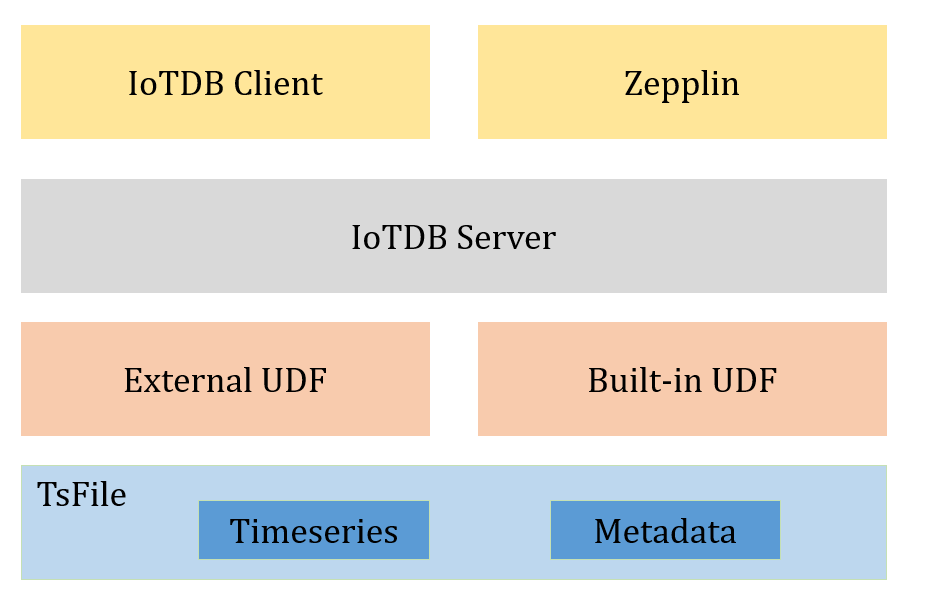
\includegraphics[width=0.66\linewidth]{udf-structure.PNG}
    \caption{基于IoTDB实现的对称模式挖掘算法架构图}
    \label{fig:symmetry_structure}
\end{figure}

% IoTDB为用户提供了一套成熟的函数管理和执行框架,本文的算法实现即基于此框架。
Apache IoTDB为用户提供了一套成熟的函数管理和执行框架,
其底层存储方式也非常方便用户对查询计算功能进行扩展。
如图~\ref{fig:symmetry_structure}所示,IoTDB的数据存储
文件TsFile中不仅存储了时间序列,还存储了与计算查询相关的元数据信息。
根据算法流程对这些数据进行有选择地应用,即可实现原生UDF和
外部UDF两种不同的计算函数。最终这两类UDF都会整合到
IoTDB Server中为用户提供相关的数据分析功能,并将结果
由命令行客户端或Apache UI工具Zepplin进行展示。
根据全局和分段对称模式挖掘算法的计算方式和数据依赖,
本章对全局算法实现了只基于原始时序数据的外部UDF,
而对分段算法则实现了外部UDF和基于元数据的原生UDF两类函数,
尽可能满足不同场景用户的计算需求。


\section{全局对称模式挖掘算法实现}
IoTDB为用户提供了一个用于时间序列数据分析的自定义模板函数接口UDTF
(User Defined Timeseries Generating Function),
该模板支持多条时间序列和多个参数的输入,最终会输出一条时间序列数据
表示函数计算的结果。对于全局对称模式算法而言,根据
图~\ref{fig:global_algorithm_process}所示的计算流程,
只需要输入一条完整的时间序列数据用于挖掘对称模式,具体的
全局对称性度量和对称度阈值确定都可以在函数处理中由算法确定。
在具体实现中,为方便用户使用,本算法提供了阈值(threshold)参数,
可以由领域专家自行指定对称度阈值,若不指定,则采用对称度阈值确定算法进行计算。
\begin{figure}
    \centering
    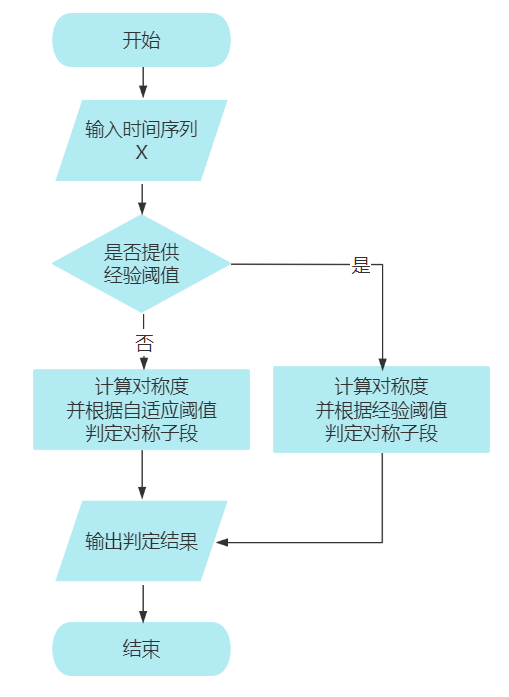
\includegraphics[width=0.55\linewidth]{global_symmetry_algorithm.PNG}
    \caption{全局对称模式挖掘算法流程图}
    \label{fig:global_algorithm_process}
\end{figure}

本算法用到了UDTF中定义的四个接口,具体实现方式如下所示:
\begin{itemize}
\item validate:验证算法的参数是否输入正确,threshold代表时间序列的
      对称度,一定是正数。如果不输入,则代表使用自定义的对称度阈值确定算法。
\item beforeStart:指定滑动窗口的数据访问策略并执行算法的初始化。由于
      全局对称模式挖掘算法是对时间序列整体计算对称性,因此,设定时间序列的
      窗口大小为无穷大以将全部数据加载到算法中。
\item transform:执行全局算法以挖掘对称模式,具体步骤如下所示:
    \begin{enumerate}
        \item 对长度小于2的时间子序列的对称度进行初始化计算。
        \item 按照长度由小到大的顺序推导并计算每一段时间子序列的对称度,并将结果
              保存在预定义的数据结构中。
        \item 根据时间序列的数据特征进行差分计算,得到对称度阈值。
        \item 由计算得到的全局对称度和对称度阈值判定输入时间序列是否属于对称模式。
    \end{enumerate}
\item terminate:将全局时间序列是否具有对称性的判定结果输出到collector中。
\end{itemize}

\section{分段对称模式挖掘算法实现}

分段对称模式挖掘算法的处理过程和全局对称模式挖掘算法有所不同,
分段算法是通过将时间序列划分为不同的子段分别挖掘对称模式的。
结合IoTDB将整条时间序列数据划分为不同的Chunk和Page进行存储,
并在计算时分段计算再合并结果的处理方式,分段算法和IoTDB的存储
计算框架高度契合。正因如此,分段算法既可以像全局算法一样
以外部UDF的方式完成计算,也可以利用每个Page的元数据加速计算。
分段对称模式挖掘算法的外部UDF实现方式非常简单,
直接利用算法~\ref{alg:symmetric_pattern}计算即可。
但分段算法的原生UDF实现方式却需要在计算时考虑元数据,
计算流程较为复杂。

\begin{figure}
    \centering
    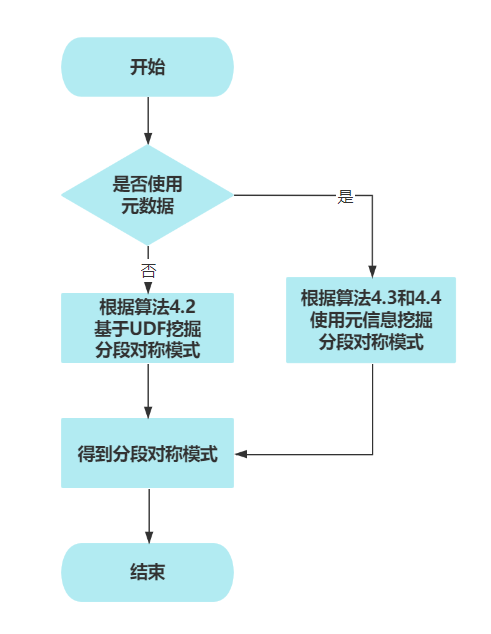
\includegraphics[width=0.55\linewidth]{iotdb_segement_symmetry.PNG}
    \caption{基于IoTDB的分段对称模式挖掘流程}
    \label{fig:iotdb_segement}
  \end{figure}

图~\ref{fig:iotdb_segement}展示了基于IoTDB的分段对称模式
挖掘算法流程。算法在读入时间序列$X$和子序列长度约束$w$之后,
首先需要判断是否存在可以利用的元数据。
元数据的可用性必须满足三个条件,一是
在写入时已完成元数据计算并持久化到TsFile中,
二是写入时从系统配置中读取的子序列长度约束必须和输入的约束$w$
相同,三是查询的范围必须包含完整Page。
经过可用性检验,如果有对应的元数据,则直接合并元数据
就可以得到分段模式的数量。
反之,则还需要重新根据算法4.2加载原始时间序列并挖掘
分段对称模式。最终,算法输出分段对称模式挖掘得到的数量结果。

% 元数据的可用性必须满足三个条件,一是
% 在写入过程中完成计算并持久化到TsFile中,另一个是
% 查询的范围必须包含完整Page。尽管Page中存在元数据但查询时
% 若并未包含Page中所有的时间序列,则仍然需要加载原始数据挖掘对称模式。

% 此外,若要使用


% 因此,在本算法的实现中,对于每一个分段对称模式,算法只输出
% 对称模式的起始时间点和其对称度信息,具体的计算流程如下所示:
% \begin{enumerate}
%     \item 首先,IoTDB通过序列读取器读取时间序列数据,
%     由于需要根据全部子序列的对称度特征进行阈值划分,
%     所以要把所有的数据全部加载到内存中,保存在算法的
%     自定义数据结构中。
%     \item 然后,在transformer函数中定义动态规划
%     状态信息,按照区间由小到大的顺序计算所有长度小于w的
%     子序列的对称度。需要注意的是,由于输出时需要明确分段模式
%     的起始时间,所以需要将RowWindow中每个时间子序列的
%     起始点时间信息保存下来。
%     \item 对transformer函数中保存的数据值进行差分计算,求得
%     相邻点距离的平均值。再采用流式算法计算子序列对称度的方差,
%     根据方差之和最大原则寻找自然断点。利用上述两个阈值候选的最小值
%     求得分段对称模式的真实阈值。
%     \item 根据贪心策略计算出数量最多的对称模式,并将结果循环输出到
%     collector中。
% \end{enumerate}

\section{算法查询展示}

在实现了对称模式挖掘的算法逻辑之后,用户可以使用两种方式
执行算法并对结果进行查询。一种是利用IoTDB-Client命令行,
另一种是在Apache Zepplin上通过前端UI进行查询。
以全局对称模式挖掘数据集和算法为例,
在命令行上,用户登录客户端之后,直接输入调用UDF函数的SQL语句
进行查询,查询结果如图~\ref{fig:iotdb_client_symptn}所示。
直接使用Select语句就可以查询全局和分段对称模式的挖掘结果。
使用IoTDB Client命令行进行查询的好处是查询便捷,
直接登陆客户端即可查询,不需要重新部署其他工具。
但是,在命令行查询的结果只能通过表格的方式
进行展示,不方便直观的观察查询结果。仅通过在命令行中观察,
用户无法区分~\ref{fig:gsymptn_input}所示的查询数据是否
具有对称性,因而更无法对查询结果的正确性进行判断。
基于此,在IoTDB-Client上进行查询只适用于开发中的结果验证,
不适合商业化用户使用。因此,需要配置部署一个直观的前端查询方式。
\begin{figure}
    \centering
    \subcaptionbox{GunPoint数据集\label{fig:gsymptn_input}}
    {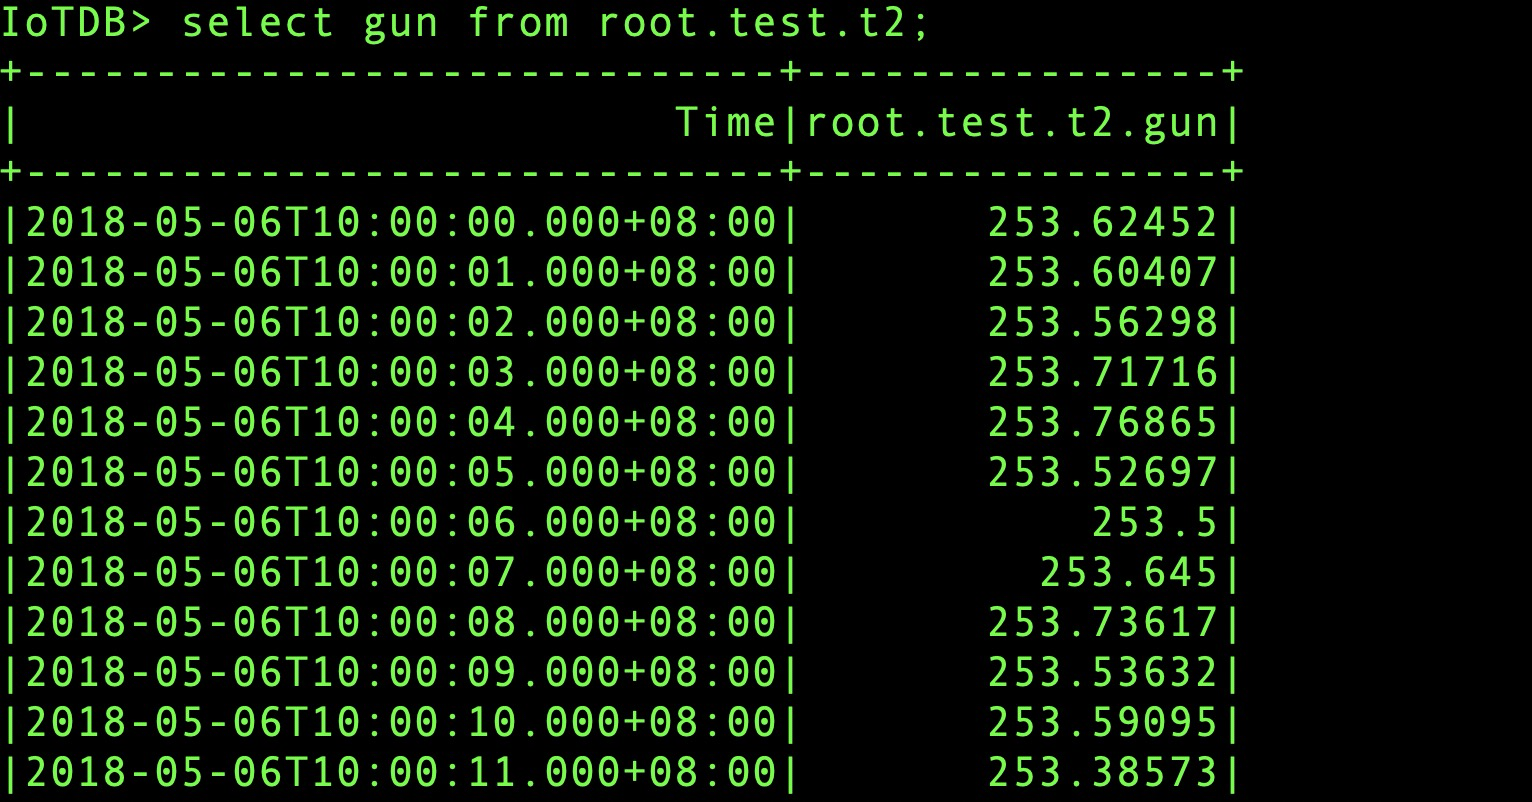
\includegraphics[width=0.76\linewidth]{gun_point_system.png}}
    \subcaptionbox{全局对称模式查询结果\label{fig:gsymptn_output}}
    {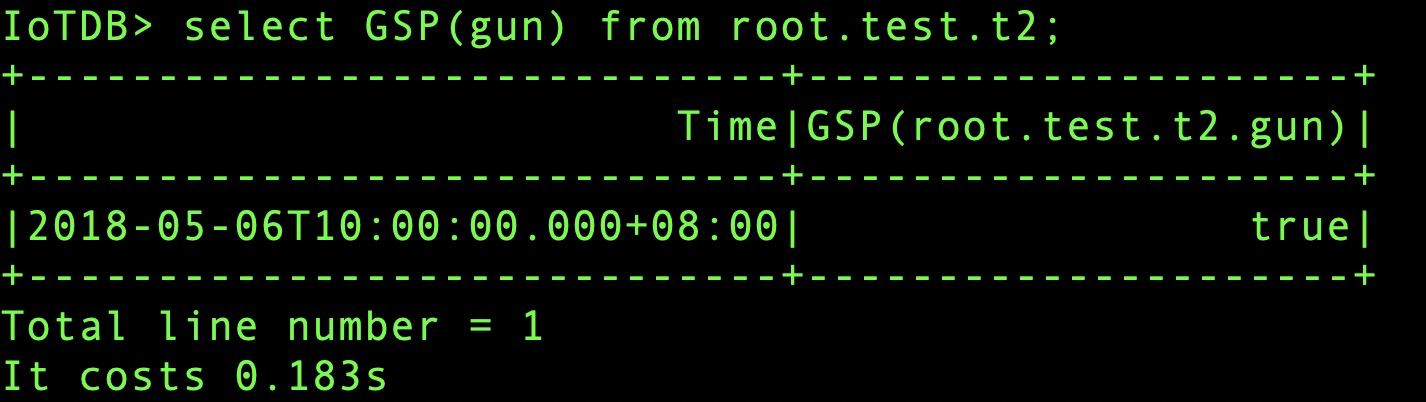
\includegraphics[width=0.76\linewidth]{gun_point_system_result.png}}
    \caption{在IoTDB-Client运行全局对称模式挖掘算法的结果查询展示}
    \label{fig:iotdb_client_symptn}
\end{figure}

Apache Zepplin是一个是一个基于网页的交互式数据分析系统。
用户可以通过Zeppelin连接IoTDB数据源并使用SQL进行交互式查询操作。
图~\ref{fig:iotdb_zepplin_symptn}中展示了在Zepplin上进行
分段对称模式挖掘结果计算并查询的方式,
图中上半部分是在运输车轨迹GPS经度
数据集随时间的变化情况。利用Zepplin自带的折线图
用户可以方便的观察出运输车轨迹数据集中的时间序列具有
16个分段对称模式。
图中下半部分是在运输车轨迹数据集上挖掘分段对称模式,
在Zepplin的输入框中直接输入Select语句
就可以像IoTDB-Client命令行一样执行查询,
发现算法的计算结果和真实结果一致。
\begin{figure}
    \centering
    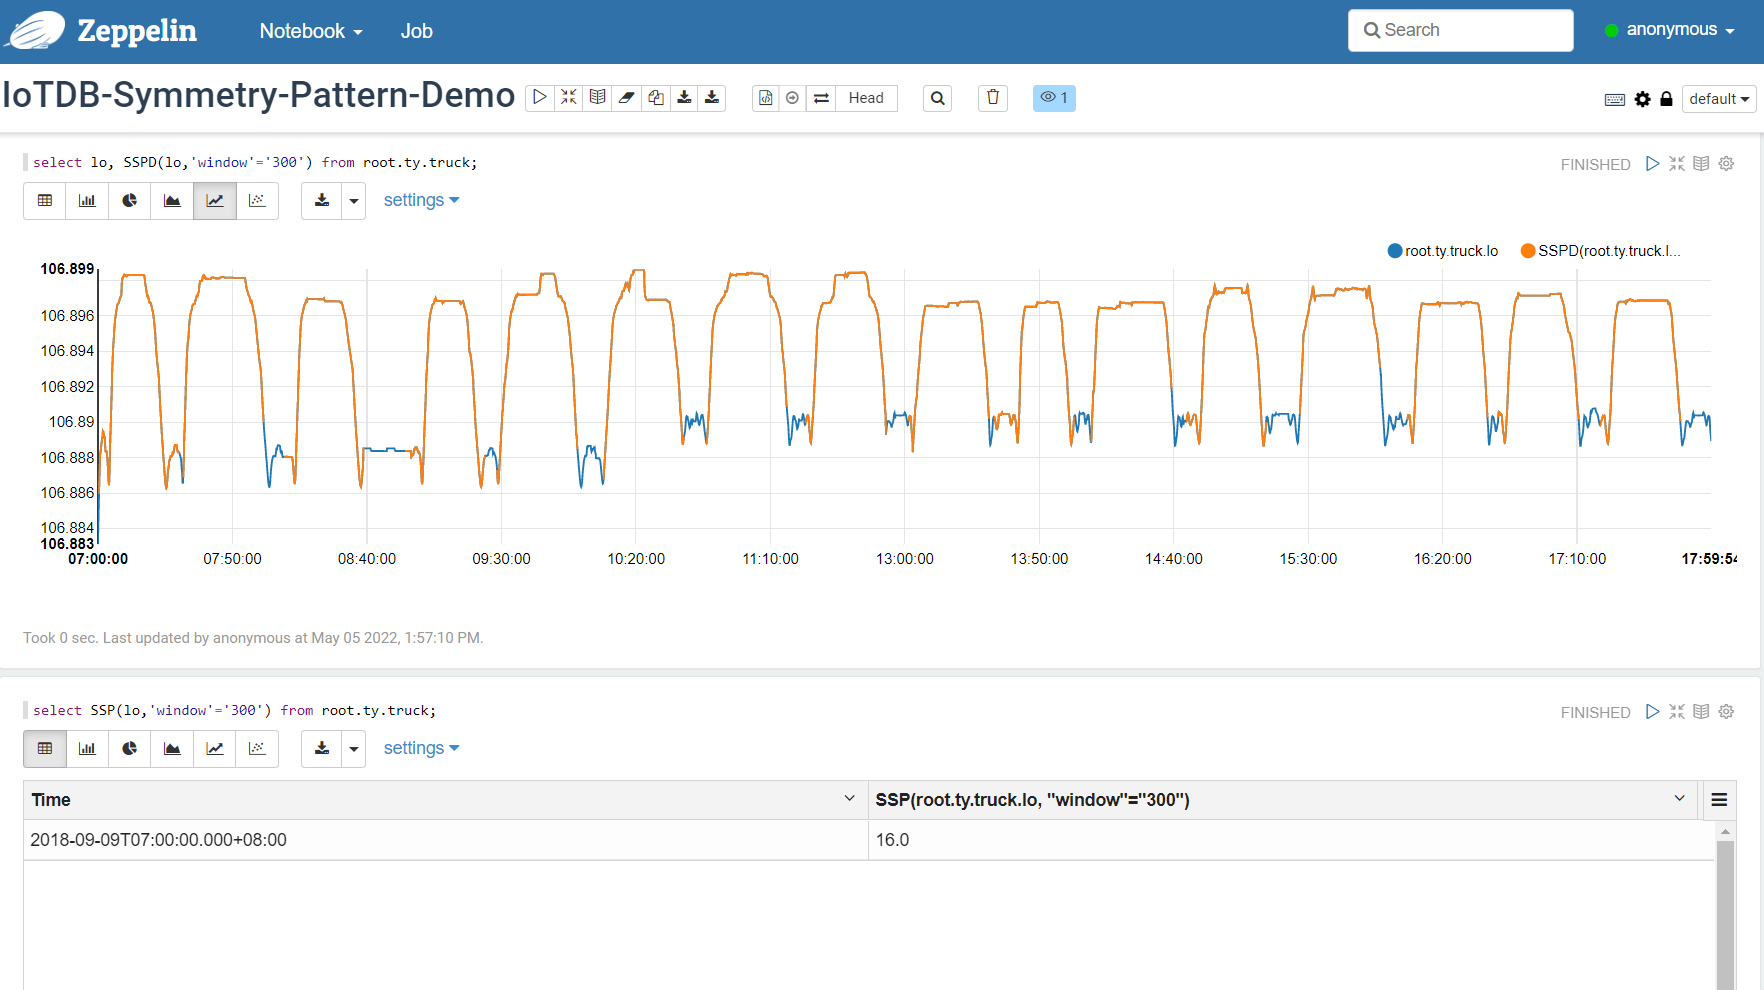
\includegraphics[width=0.86\linewidth]{zepplin_truck_data.PNG}
    \caption{在Apache zepplin运行分段对称模式挖掘算法的结果查询展示}
    \label{fig:iotdb_zepplin_symptn}
\end{figure}


\section{本章小结}
本章主要介绍了根据IoTDB提供的用户自定义函数模板接口,
全局对称模式挖掘算法和分段对称模式挖掘算法的实现方式,
并通过在IoTDB Server上进行部署,使用IoTDB Client和
Apache Zepplin两种方式进行函数调用计算和结果查询。
通过基于IoTDB实现这两种算法,弥补了IoTDB Quality挖掘对称模式
的功能缺失,在帮助用户得到蕴含在时间序列中对称特征的同时,
便于发现违反模式规律的异常点并进行检测和修复。